\documentclass[11pt]{article}

% Change "review" to "final" to generate the final (sometimes called camera-ready) version.
% Change to "preprint" to generate a non-anonymous version with page numbers.
\usepackage[final]{acl}

% Standard package includes
\usepackage{times}
\usepackage{latexsym}

% For proper rendering and hyphenation of words containing Latin characters (including in bib files)
\usepackage[T1]{fontenc}
% For Vietnamese characters
% \usepackage[T5]{fontenc}
% See https://www.latex-project.org/help/documentation/encguide.pdf for other character sets

% This assumes your files are encoded as UTF8
\usepackage[utf8]{inputenc}

% This is not strictly necessary, and may be commented out,
% but it will improve the layout of the manuscript,
% and will typically save some space.
\usepackage{microtype}

% This is also not strictly necessary, and may be commented out.
% However, it will improve the aesthetics of text in
% the typewriter font.
\usepackage{inconsolata}

% Including images in your LaTeX document requires adding
% additional package(s)
\usepackage{graphicx}
% Allow breakable verbatim blocks
\usepackage{fancyvrb}

% If the title and author information does not fit in the area allocated, uncomment the following
%
%\setlength\titlebox{<dim>}
%
% and set <dim> to something 5cm or larger.
\setlength\titlebox{7.5cm}

\title{RAG for Image Captioning}

% Author information can be set in various styles:
% For several authors from the same institution:
% \author{Author 1 \and ... \and Author n \\
%         Address line \\ ... \\ Address line}
% if the names do not fit well on one line use
%         Author 1 \\ {\bf Author 2} \\ ... \\ {\bf Author n} \\
% For authors from different institutions:
% \author{Author 1 \\ Address line \\  ... \\ Address line
%         \And  ... \And
%         Author n \\ Address line \\ ... \\ Address line}
% To start a separate ``row'' of authors use \AND, as in
% \author{Author 1 \\ Address line \\  ... \\ Address line
%         \AND
%         Author 2 \\ Address line \\ ... \\ Address line \And
%         Author 3 \\ Address line \\ ... \\ Address line}

\author{Saravanan S \\ 24210090 \\ IIT Gandhinagar \\
  \texttt{24210090@iitgn.ac.in}
  \And
  Maharshi Patel \\ 24210059 \\ IIT Gandhinagar \\
  \texttt{maharshi.patel@iitgn.ac.in}
  \And
  Harsh Verma \\ 24250039 \\ IIT Gandhinagar \\
  \texttt{harsh.verma@iitgn.ac.in}
  \AND
  Abhiroop Chintalapudi \\ 24250007 \\ IIT Gandhinagar \\
  \texttt{abhiroop.chintalapudi@iitgn.ac.in}
  \And
  Mithlesh Singla \\ 24210063 \\ IIT Gandhinagar \\
  \texttt{mitlesh.singla@iitgn.ac.in}
  \AND
  Uday Sankar Gottipalli \\ 24210108 \\ IIT Gandhinagar \\
  \texttt{uday.gottipalli@iitgn.ac.in}
  \And
  Abhay Pisharodi \\ 24290001 \\ IIT Gandhinagar \\
  \texttt{abhay.pisharodi@iitgn.ac.in}
}

%\author{
%  \textbf{First Author\textsuperscript{1}},
%  \textbf{Second Author\textsuperscript{1,2}},
%  \textbf{Third T. Author\textsuperscript{1}},
%  \textbf{Fourth Author\textsuperscript{1}},
%\\
%  \textbf{Fifth Author\textsuperscript{1,2}},
%  \textbf{Sixth Author\textsuperscript{1}},
%  \textbf{Seventh Author\textsuperscript{1}},
%  \textbf{Eighth Author \textsuperscript{1,2,3,4}},
%\\
%  \textbf{Ninth Author\textsuperscript{1}},
%  \textbf{Tenth Author\textsuperscript{1}},
%  \textbf{Eleventh E. Author\textsuperscript{1,2,3,4,5}},
%  \textbf{Twelfth Author\textsuperscript{1}},
%\\
%  \textbf{Thirteenth Author\textsuperscript{3}},
%  \textbf{Fourteenth F. Author\textsuperscript{2,4}},
%  \textbf{Fifteenth Author\textsuperscript{1}},
%  \textbf{Sixteenth Author\textsuperscript{1}},
%\\
%  \textbf{Seventeenth S. Author\textsuperscript{4,5}},
%  \textbf{Eighteenth Author\textsuperscript{3,4}},
%  \textbf{Nineteenth N. Author\textsuperscript{2,5}},
%  \textbf{Twentieth Author\textsuperscript{1}}
%\\
%\\
%  \textsuperscript{1}Affiliation 1,
%  \textsuperscript{2}Affiliation 2,
%  \textsuperscript{3}Affiliation 3,
%  \textsuperscript{4}Affiliation 4,
%  \textsuperscript{5}Affiliation 5
%\\
%  \small{
%    \textbf{Correspondence:} \href{mailto:email@domain}{email@domain}
%  }
%}

\begin{document}
\maketitle
%\begin{abstract}
%This document is a supplement to the general instructions for *ACL authors. It contains instructions for using the \LaTeX{} style files for ACL conferences.
%The document itself conforms to its own specifications, and is therefore an example of what your manuscript should look like.
%These instructions should be used both for papers submitted for review and for final versions of accepted papers.
%\end{abstract}

\section{Report}
\label{sec:report}

This report follows the assignment specification (CS 613: Natural Language Processing) for project. The source code for our experiments will be available at \href{https://github.com/shadowscythe03/RAG_Image_Captioning}{here}

\subsection{Feedback and Novelties (10 Pts)}
Since the first presentation, our team initially proposed to implement a multilingual image captioning RAG (Retrieval-Augmented Generation) model and make modifications to its architecture. However, based on the professor's feedback, we shifted our focus more towards improving the architecture of the RAG model itself instead of expanding it to multiple languages at this stage.

During our mentor discussions, it was suggested that we carefully analyze the baseline paper's implementation to identify the main bottlenecks and understand where improvements could be made. Through this process, we found that the baseline model had limitations in representing multiple objects within an image, which affected the quality of the generated captions and the retrieval results. We also noticed potential inefficiencies in the nearest embedding search algorithm and the way visual features were encoded.

To address these issues, we started working on enhancing the image representation by integrating object detection and segmentation algorithms. This allowed us to detect multiple objects in a single image and generate individual embeddings for each object using CLIP. We then combined these embeddings to form a more comprehensive image representation, which was later used for searching and retrieving relevant information from the database. By doing this, we aimed to overcome the issue of limited object representation and improve the overall performance of the RAG model.

Throughout our weekly meetings, we continuously refined this approach, discussed various design choices, and compared the results of our modified architecture with the baseline outcomes.

\textbf{Key novelties implemented:}
\begin{itemize}
  \item \textbf{Multi-object representation:} Integration of DETR-based object detection and semantic segmentation to identify and encode individual objects/regions within images
  \item \textbf{Enhanced retrieval context:} Generation of crop-specific embeddings that are individually queried against the ChromaDB database, providing richer contextual information
  \item \textbf{Vision-language generation:} Implementation of BLIP-2 for caption generation conditioned on both visual input and retrieved textual context
  \item \textbf{Ablation-ready architecture:} Three distinct approaches (original RAG, aggregation-based, and full vision-language) enabling systematic performance comparison
\end{itemize}


\subsection{Baselines and State-of-the-Art (10 Pts)}
We will compare against the following baselines and SOTA papers:
\begin{itemize}
  \item DIR ("DIR: Retrieval-Augmented Image Captioning with Comprehensive Understanding" by Hao Wu et al.) — described in our template as the current state-of-the-art for robust retrieval-augmented image captioning. DIR improves image representations using diffusion guidance; code was not available to us.
  \item SmallCap — available implementation; used as a practical baseline since DIR and other SOTA models build on SmallCap.
  \item RobustCap — we attempted to run the available code but were unable to get it working reliably; it remains a potential competitor if we resolve environment issues.
\end{itemize}

Baseline implementation availability: for this project, SmallCap code is available and used; DIR code is not available, so we re-implement comparable components where feasible.

\begin{table*}[t]
  \centering
  \begin{tabular}{|l|c|c|c|c|c|}
    \hline
    Method                       & Train Data & Flickr30k & NoCaps Val & Out-domain & Overall \\
    \hline
    Heavyweight training methods &            &           &            &            &         \\
    BLIP [17]                    & 129M       & 446B      & -          & -          & 115.3   \\
    BLIP2 [18]                   & 129M       & 1.2B      & -          & -          & 124.8   \\
    ViECap [12]                  & COCO       & 124M      & 47.9       & 13.6       & 66.2    \\
    \hline
    Lightweight training methods &            &           &            &            &         \\
    MiniGPT4 [40]                & 5M         & 3.94M     & 78.4       & 16.9       & 110.8   \\
    ClipCap [24]                 & COCO       & 43M       & -          & -          & 49.1    \\
    SmallCap [29]                & COCO       & 7M        & 60.6       & -          & -       \\
    EVCap [19]                   & COCO       & 3.97M     & 84.4       & 18.0       & 116.5   \\
    DIR (ours)                   & COCO       & 3.97M     & 85.7       & 18.2       & 120.7   \\
    \hline
  \end{tabular}
  \caption{Summary of methods and their performance metrics.}
  \label{tab:methods_performance}
\end{table*}

\subsection{Datasets (5 Pts)}
Primary datasets and handling:
\begin{itemize}
  \item COCO dataset (common choice for image captioning). Use standard train/val/test splits unless otherwise noted.
  \item Dataset Size: 243429 Captions
  \item Images: 40505
  \item Captions: 243429
  \item Avg Captions per image: 5
  \item Vocabulary size: 17,039 (as reported for COCO in related work).
        %  \item Bias handling: document sampling biases (object frequency, scene bias) and mitigation strategies (balanced sampling, augmentation, or additional dataset curation).
        %  \item Dataset extensions: if we extend COCO (e.g., include object-level annotations or external textual knowledge for retrieval), describe differences and the augmentation pipeline.
\end{itemize}

\subsection{Experimental Plan (15 Pts)}
Our Experimental Plan
\begin{itemize}
  %  \item Training setup: hardware (GPU model, memory), batch sizes, learning rate schedules, number of epochs, checkpointing policy.
  \item Models/approaches:
        \begin{itemize}
          \item Used ChromaDB for Retrieval-Augmented-Generation(RAG)
          \item Used \texttt{facebook/detr-resnet-50} and \texttt{facebook/detr-resnet-50-panoptic} for object detection and segmentation
          \item \texttt{Salesforce/blip2-opt-2.7b} for Generating captions from images
        \end{itemize}
  \item Each crop is sent to the database and captions are retrieved which are then sent to the LLM for captioning.
        %  \item Parameter counts and architecture differences: report model parameter counts and highlight what changes increased/decreased capacity.
        %  \item Hyperparameter search strategy: grid search for small sweeps, or Bayesian/Successive Halving for more efficient tuning; include ranges tested.
        %  \item Ablation table plan: prepare tables that compare metrics across variants (with/without object embeddings, different retrieval indices, different encoder heads).
        %  \item Metrics: BLEU, METEOR, ROUGE\_L, CIDEr, SPICE. Rationale: these are standard in captioning literature and capture lexical and semantic quality.
        %  \item Additional metrics: consider human evaluation, grounding metrics, or retrieval-specific metrics (recall@k) if applicable.
\end{itemize}

\subsection{Project Management (10 Pts)}
Team organisation and resources:
\begin{itemize}
  \item Proposed novel solutions generation: iterative design based on baseline analysis, mentor feedback, and small-scale experiments.
  \item Compute resources: Used Colab and Singularity for Resources.
  \item Task distribution: Shared by Everyone.
\end{itemize}

\section{Experiment}
\label{sec:experiment}

This section summarises the implementation and evaluation plan from the assignment prompt.

\subsection{Implementation (50 Pts)}
We implemented a complete RAG-based image captioning pipeline with the following key components:

\textbf{Core Architecture:}
\begin{itemize}
  \item \textbf{Embedding Model:} CLIP (ViT-B-32) for image and region encoding
  \item \textbf{Retrieval Database:} ChromaDB populated with 10,000 COCO training image embeddings
  \item \textbf{Vision-Language Model:} BLIP-2 (\texttt{Salesforce/blip2-opt-2.7b}, 2.7B parameters) for caption generation conditioned on image and retrieved context
\end{itemize}

\textbf{Advanced Image Understanding:}
\begin{itemize}
  \item \textbf{Object Detection:} DETR (\texttt{facebook/detr-resnet-50}) to extract salient object regions
  \item \textbf{Semantic Segmentation:} DETR Panoptic (\texttt{facebook/detr-resnet-50-panoptic}) for region-based crops
  \item \textbf{Multi-region Retrieval:} Each detected object/segment crop is individually encoded, captions retrieved, and aggregated with original image retrievals
\end{itemize}

\textbf{Three Evaluated Approaches:}
\begin{itemize}
  \item \textbf{Original RAG:} Retrieval from original image only → BLIP-2 generation
  \item \textbf{Proposed RAG (Aggregation):} Text concatenation of original + crop-level retrievals (no LLM generation)
  \item \textbf{Proposed RAG + BLIP-2:} Full vision-language generation using original + crop retrievals as contextual input
\end{itemize}

\textbf{Technical Optimizations:}
\begin{itemize}
  \item Memory management: 8-bit quantization support, aggressive GPU cache clearing, reduced beam search (3 beams)
  \item GPU requirements: ~6GB (without DETR), ~16GB (with DETR enabled)
  \item Evaluation: 1000 COCO val2017 images, standard metrics (BLEU-1/2/3/4, METEOR, ROUGE-L, CIDEr) via \texttt{pycocoevalcap}
        % \item Automated output: Timestamped CSV results and visualization samples
\end{itemize}

\subsection{Reporting Results and Findings (10 Pts)}
The following figure shows a comparison of the performance metrics between the two proposed RAG variants (Proposed RAG (Original + Crops) and RAG) across standard evaluation metrics.

\begin{figure*}[!t]
  \centering
  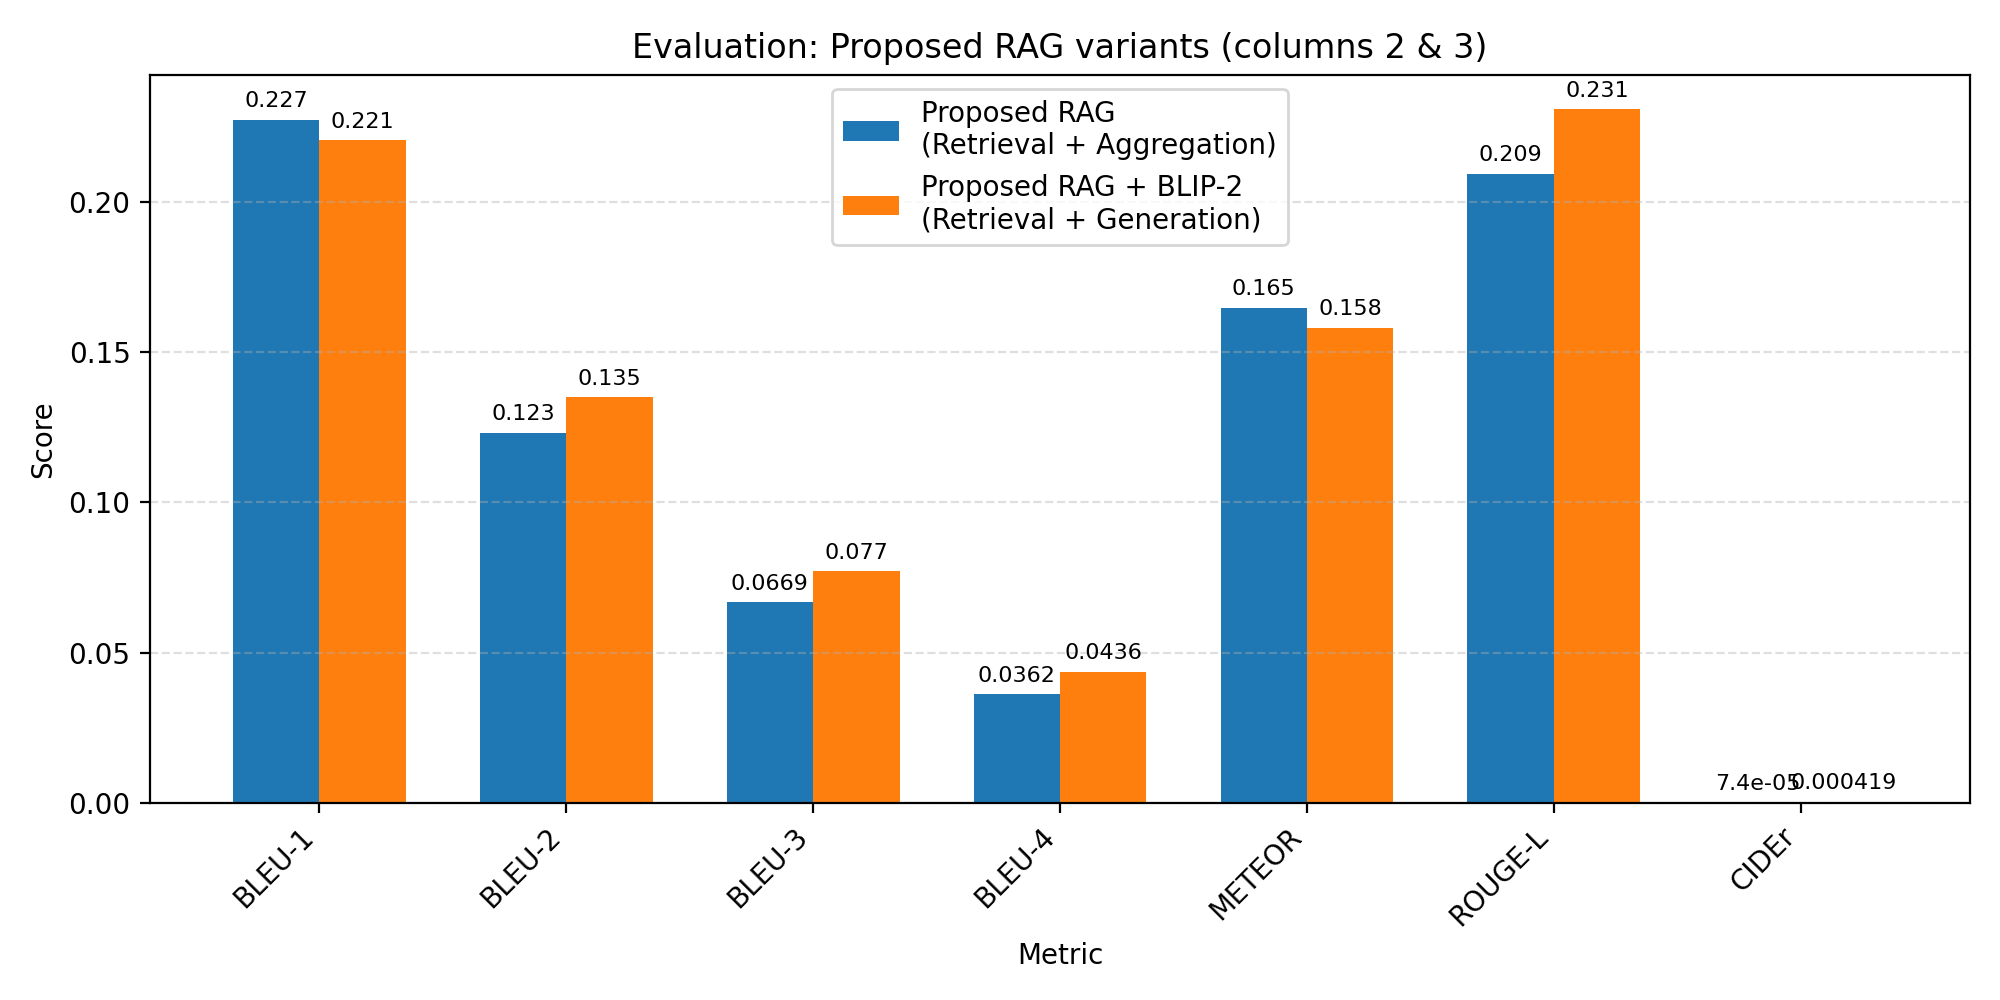
\includegraphics[width=0.7\textwidth]{plot_columns_2_3.png}
  \caption{Performance comparison between Proposed RAG variants across evaluation metrics (BLEU, METEOR, ROUGE-L, CIDEr). The chart shows the quantitative results for both the Original+Crops approach and the Crops-only approach.}
  \label{fig:results_comparison}
\end{figure*}

\subsubsection{Sample results}
Below we provide two representative qualitative examples from our experiments. Each example shows the original retrieved captions (Original RAG), the crop-level captions and the final aggregated caption using the Proposed RAG (Original + Crops).

\paragraph{Example 1 -- Image 000000261982.jpg}

\textbf{Original retrieved captions (Original RAG):}\ref{fig:sample1}
\begin{quote}
  ``A skateboarder is riding his skateboard at night. A young man riding a skateboard on a street. A skateboarder wearing a plaid shirt and jeans. A skate boarder at night prepairing to skate away.''
\end{quote}

\textbf{Proposed RAG (Original + Crops):}
\begin{quote}
  \textbf{Number of Crops Generated:} 4

  \textbf{Crop Captions:}
  \begin{itemize}
    \item \textbf{Crop 1:} A skateboarder is riding his skateboard at night. A young man riding a skateboard on a street. A skate boarder at night prepairing to skate away.
    \item \textbf{Crop 2:} A tabby house cat walking all over it's owner. Cat sitting on the stomach of a woman laying down on a bed. A cat looking down at the person lying on the bed.
    \item \textbf{Crop 3:} A skateboarder is riding his skateboard at night. A young man riding a skateboard on a street. A skateboarder wearing a plaid shirt and jeans.
    \item \textbf{Crop 4:} Small grey cat crawling over a woman's stomach. Cat sitting on the stomach of a woman laying down on a bed. A cat looking down at the person lying on the bed.
  \end{itemize}

  \textbf{Final Aggregated Caption:}
  A skateboarder is riding his skateboard at night. A young man riding a skateboard on a street. A skateboarder wearing a plaid shirt and jeans. skate boarder prepairing away. tabby house cat walking all over owner. sitting the stomach woman laying down bed. looking person.
\end{quote}

\begin{figure*}[h]
  \centering
  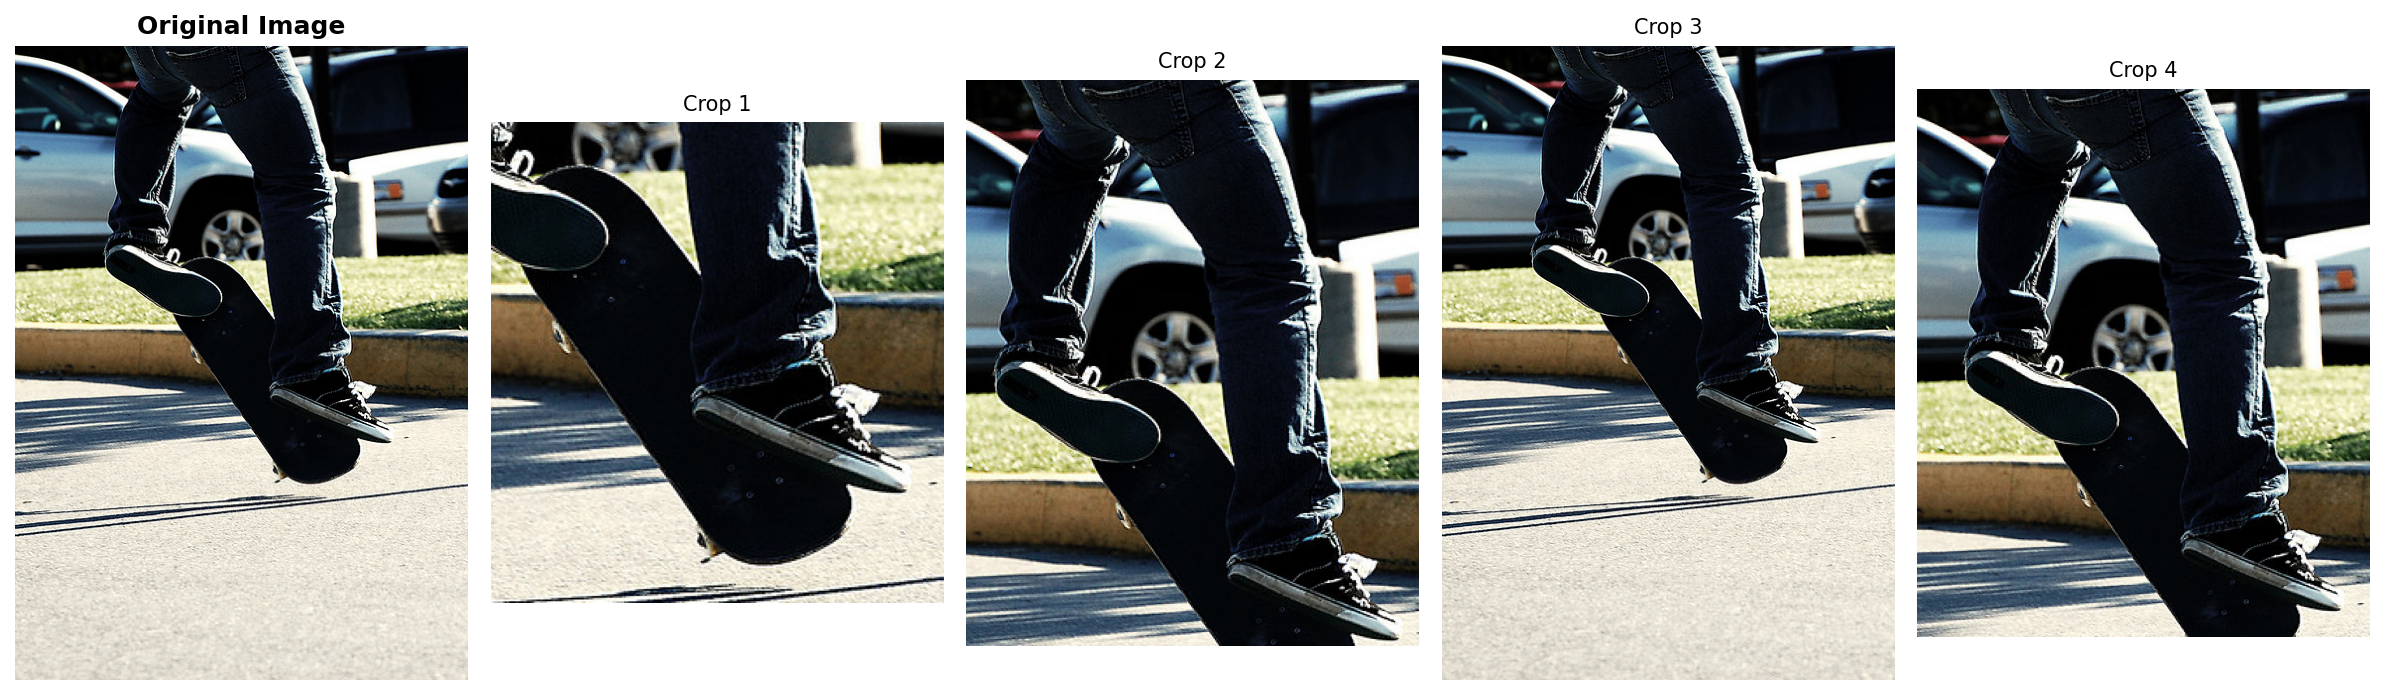
\includegraphics[width=0.9\textwidth]{evaluation_results/sample_results_20251105_215414/sample_2_visualization.png}
  \caption{Example 1 (Image 000000261982) — original image and generated crops used by the Proposed RAG aggregation.}
  \label{fig:sample1}
\end{figure*}

\paragraph{Example 2 -- Image 000000248400.jpg}\textbf{Original retrieved captions (Original RAG):}\ref{fig:sample2}
\begin{quote}
  ``A man sits on a toilet in a bathroom. A man sits on a toilet while looking at porn magazines. A person sits on the toilet in a bathroom reading a magazine. A fat ass sitting on a toilet with lady magazines.''
\end{quote}

\textbf{Proposed RAG (Original + Crops):}
\begin{quote}
  \textbf{Number of Crops Generated:} 4

  \textbf{Crop Captions:}
  \begin{itemize}
    \item \textbf{Crop 1:} A room is shown with a washer and oven. An oven, and clothes washer are in a small kitchen. a kitchen with a stove a dih washer and a mcirowave.
    \item \textbf{Crop 2:} A pizza sitting on top of a table with olives, sausage and cheese. A pizza with multiple toppings on it, including olives. The personal pizza is topped with black olives and anchovies.
    \item \textbf{Crop 3:} A bathroom with urinals that have graffiti above them. A series of urinals on a graffiti covered wall. Three urinals and another toilet in a bathroom.
    \item \textbf{Crop 4:} A dirty bathroom consisting of a toilet, bath tub and sink. a bathroom with a toilet and a sink. A bathroom mirror, with a person taking a picture in it.
  \end{itemize}

  \textbf{Final Aggregated Caption:}
  A man sits on a toilet in a bathroom. A man sits on a toilet while looking at porn magazines. A fat ass sitting on a toilet with lady magazines. room shown washer and oven. clothes are small kitchen. stove dih mcirowave pizza top table olives, sausage cheese. multiple toppings.
\end{quote}

\begin{figure*}[t]
  \centering
  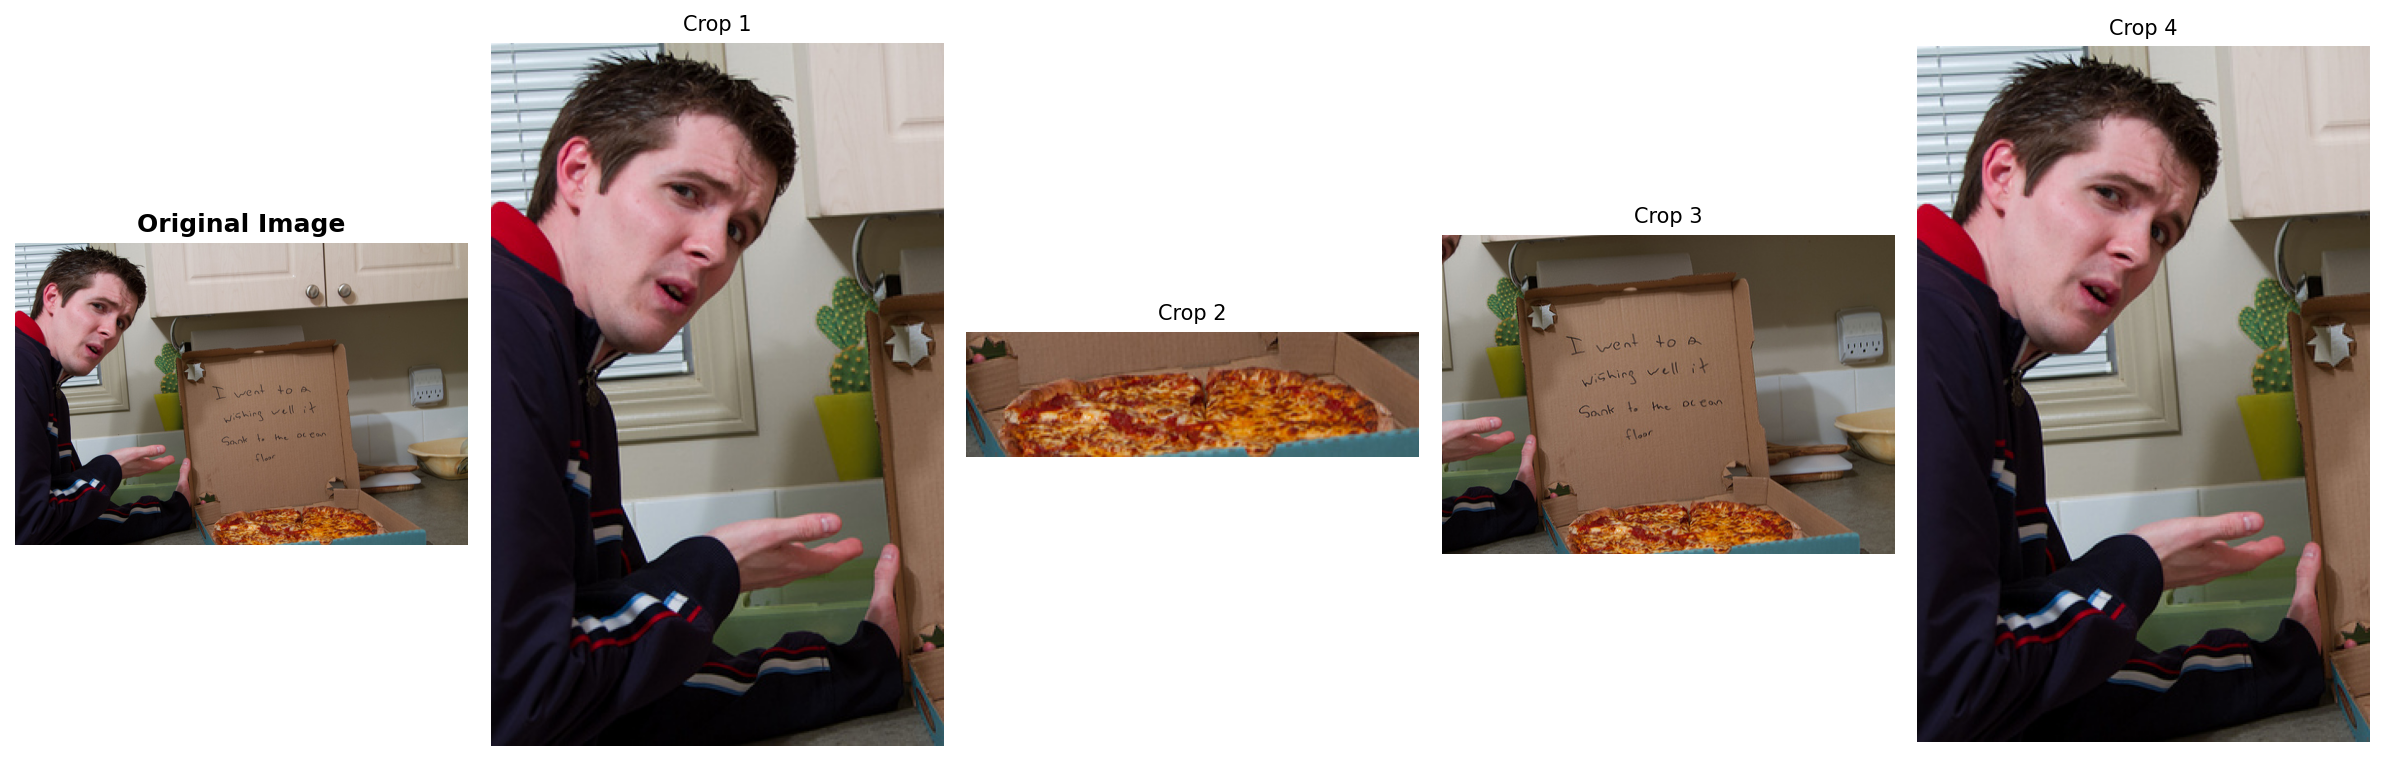
\includegraphics[width=0.9\textwidth]{evaluation_results/sample_results_20251105_215414/sample_4_visualization.png}
  \caption{Example 2 (Image 000000248400) — original image and generated crops used by the Proposed RAG aggregation.}
  \label{fig:sample2}
\end{figure*}


\subsection{Viva (40 Pts)}
Be prepared to demonstrate the code, run a small end-to-end example on a held-out image, and discuss the design choices, parameter counts, ablations, and failure cases.

\nocite{*}
\bibliography{custom}

\appendix

%\section{Implementation Notes and Checklist}
%\begin{itemize}
%  \item Add team member names and GitHub repository link in the PDF final submission.
%  \item Ensure all scripts have reproducible seeds and clear instructions for environment setup.
%  \item Include small test script to run a quick end-to-end demo (single image inference + retrieval) for the viva.
%\end{itemize}

\end{document}